\documentclass[
	letterpaper, % Use US letter paper size
]{mlreport}

\bibliography{references}

\author{Kyle Grace}
\email{kgrace6@gatech.edu}
\title{Project1 Report - Supervised Learning}

\begin{document}
%\lsstyle

\maketitle

\begin{abstract}
5 of the most popular machine learning models, Decision Trees, Boosting, Neural Networks, Support Vector Machines, and K-Nearest Neighbor, are compared with each other on 2 different datasets. They will be compared primarily on the differences of each model when it comes to training time, prediction time, and total accuracy, but there are also more nuanced details of each model discussed.
\end{abstract}

\section{Overview}
The 5 models being compared and analyzed are: Decision Trees, Boosting, Neural Networks, Support Vector Machines, and K-Nearest Neighbor. Each model has been trained and tested on 2 datasets to show how they work with different data. For each model I will also dicuss the learning curve, parameters being tuned, how changing those parameters affects the model, overall accuracy, time to train and predict using the model, and the strengths and weaknesses.

\section{Datasets}
There are 2 datasets being used for testing these models. The first dataset is a water quality model on kaggle (https://www.kaggle.com/datasets/adityakadiwal/water-potability). This dataset is a numerical dataset that associates several metrics with water "potability", which is 0 if the water is unsafe for human consumption, or 1 if it is safe. There are 9 features: ph, Hardness, Solids, Chloramines, Sulfate, Conductivity, Organic carbon, Trihalomethanes, and Turbidity, all of which are floating point values.

There are a few factors that make this dataset interesting. The primary reason is that even though it is just a binary classifier, it is still surprisingly challenging to get accurate predictions. Even though one might naturally think that a binary classifier with 9 available features would get very high accuracy models, but that hasn't been the case. At the same time, it seems to have good quality data and shows varying qualities in different models. All of this will be discussed in more detail in each section. To summarize, even though it looks easy it has been more challenging than expected.

The second dataset is also a binary classification model showing the liklihood of heart attack based on 12 health metrics (www.kaggle.com/datasets/rashikrahmanpritom/heart-attack-analysis-prediction-dataset). The 12 health metrics are: age, sex (0 or 1), cp (chest pain of 4 types), trtbps (resting blood pressure), chol (cholesterol), fbs (fasting blood sugar), restecg (resting electrocardiographic results), thalach (max heart rate), exng (exercise induced angina, 1 for yes, 0 for no), oldpeak (the previous peak), slp (slope), caa (number of major vessels), and thall (Thal rate).

I was originally going to find a different model so that I could have more variety than just 2 binary classification models, but even though at a surface level this looks similar to the water quality dataset, there are some very interested differences in performance. So in some ways, it makes the results even more interesting, since two seemingly similar models perform so differently. The two main factors that make this dataset different from the water potability dataset is that the heart data is more categorical, meaning many of the features, although represented as numbers, are actually putting the feature into a finite set of groups, where the water potability data is all continuous. As a result, I predicted that models such as decision trees and KNN would perform better on the heart data than on the water potability data.

\subsection{Performance}
\subsection{Summary}
\begin{figure}
	\centering
	{\frame{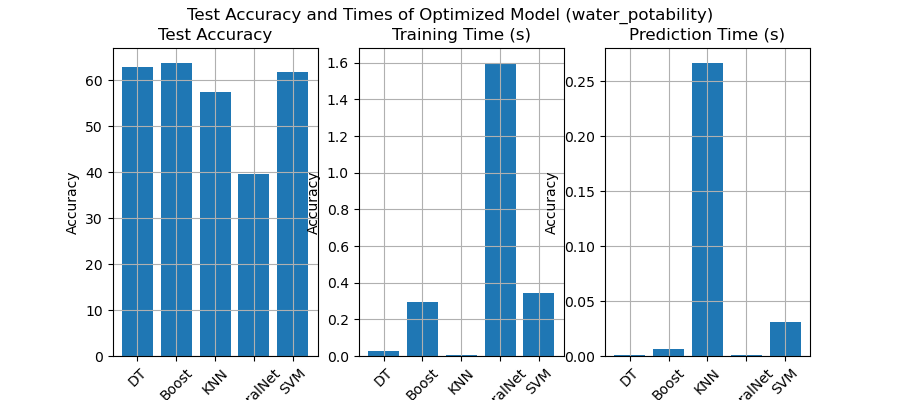
\includegraphics[width=0.90\textwidth]{../outputs/PerformanceComparison_water_potability.png}}}
	\caption{Performance comparison for the Water potability dataset. (left) Accuracy on test set (middle) Average training time (right) Average prediction time}
	\label{fig:fig1}
\end{figure}
\begin{figure}
	\centering
	{\frame{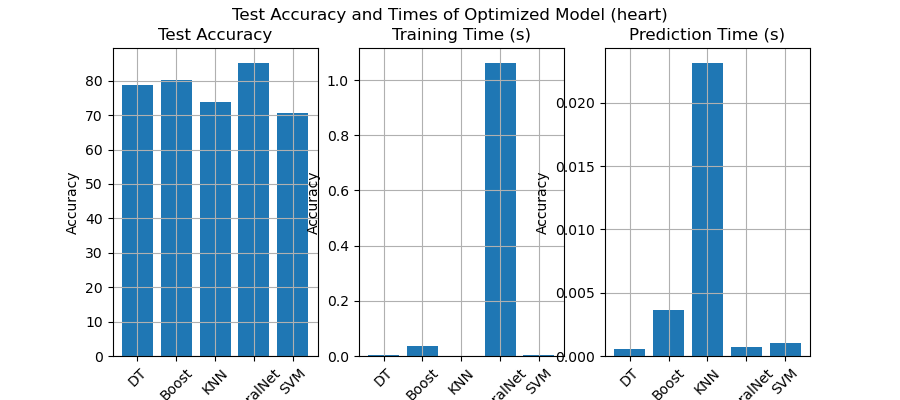
\includegraphics[width=0.90\textwidth]{../outputs/PerformanceComparison_heart.png}}}
	\caption{Performance comparison for the Heart dataset. (left) Accuracy on test set (middle) Average training time (right) Average prediction time}
	\label{fig:fig2}
\end{figure}

For figure 1 and figure 2, each model was tuned such that it acheived the highest cross-validation score, then predicted values for the test set. Both the cross-validation and test accuracy scores will be discussed further in each section, but this gives a good overview of the performance of each model.

\subsection{Decision Trees}
% TODO: Add runtimes to tables
A Decision Tree is a fairly simple model, but it turned out to be very effective. They are well suited for categorical classification, because of how they split data on different values within a feature. Integer or binned values tends to make it easier to split because the separation is more defined compared continuous values. So I expected DTs to perform well on both datasets, but not as well on the water data as the heart data. Because of the simplicity of decision trees, they are also the fastest model overall, with both training and predictions in the 2nd fastest of all models.
% accuracy table
\begin{center}
	\begin{tabular}{|c||c|c|}
	 \hline
	  & Cross Validation Score & Test Accuracy \\
	 \hline\hline
	 Water Dataset & 63.5\%  & 62.8\% \\
	 \hline
	 Heart Dataset & 78.5\%  & 78.7\% \\
	 \hline
	\end{tabular}
	\label{table:table1}
\end{center}

% Decision Tree Plots - Water
\begin{figure}
	\centering
	\subfigure[]{\frame{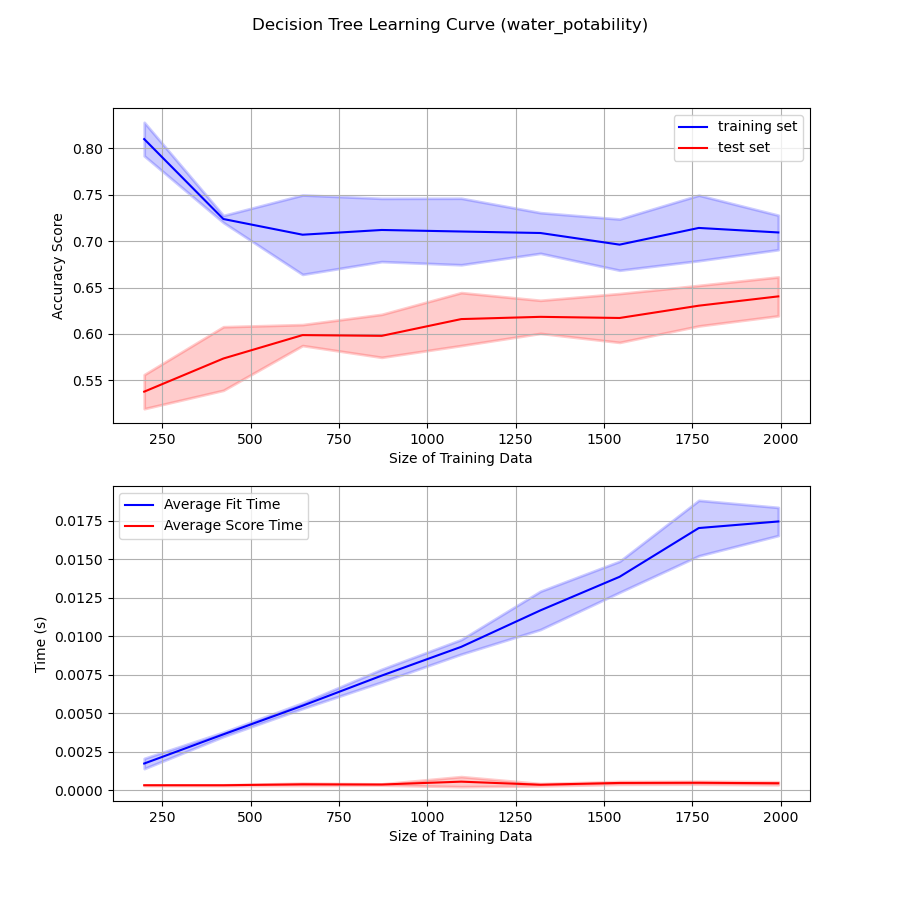
\includegraphics[width=0.40\textwidth]{../outputs/DT_LearningCurve_water_potability.png}}}
	\subfigure[]{\frame{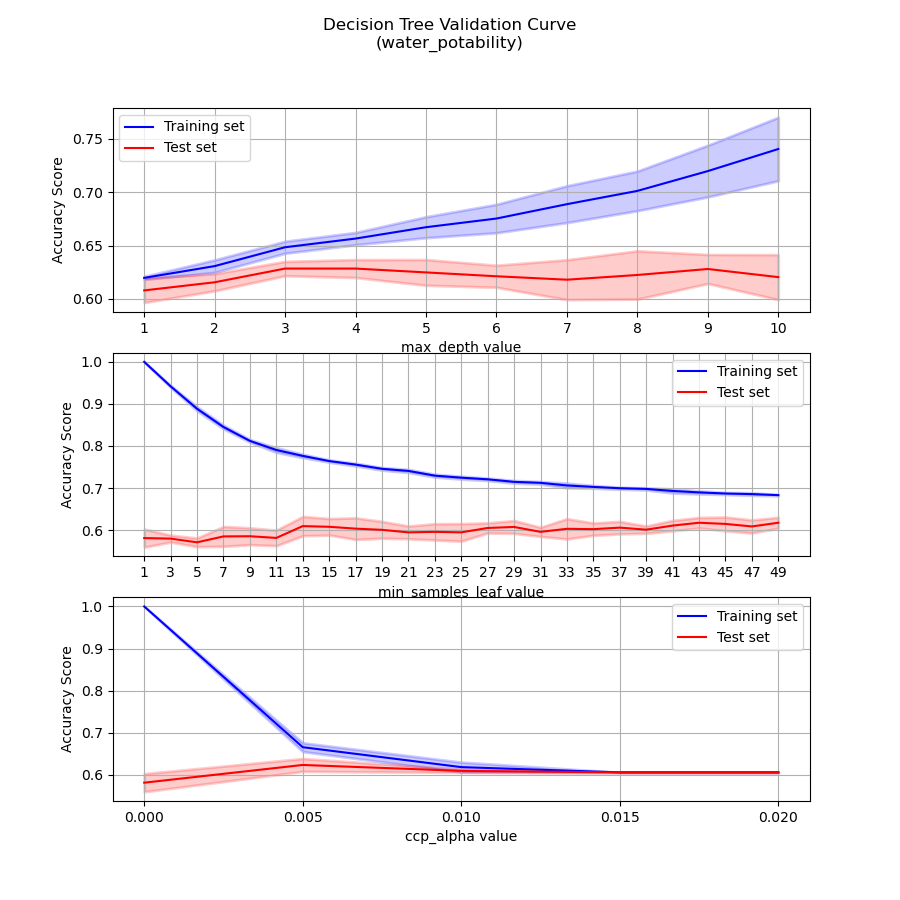
\includegraphics[width=0.40\textwidth]{../outputs/DT_ValidationCurve_water_potability.png}}}
	\caption{Decision Tree Model trained on the Water potability dataset. (a) Learning Curve and (b) Validation Curve}
	\label{fig:fig3}
\end{figure}
% Decision Tree Plots - Heart
\begin{figure}
	\centering
	\subfigure[]{\frame{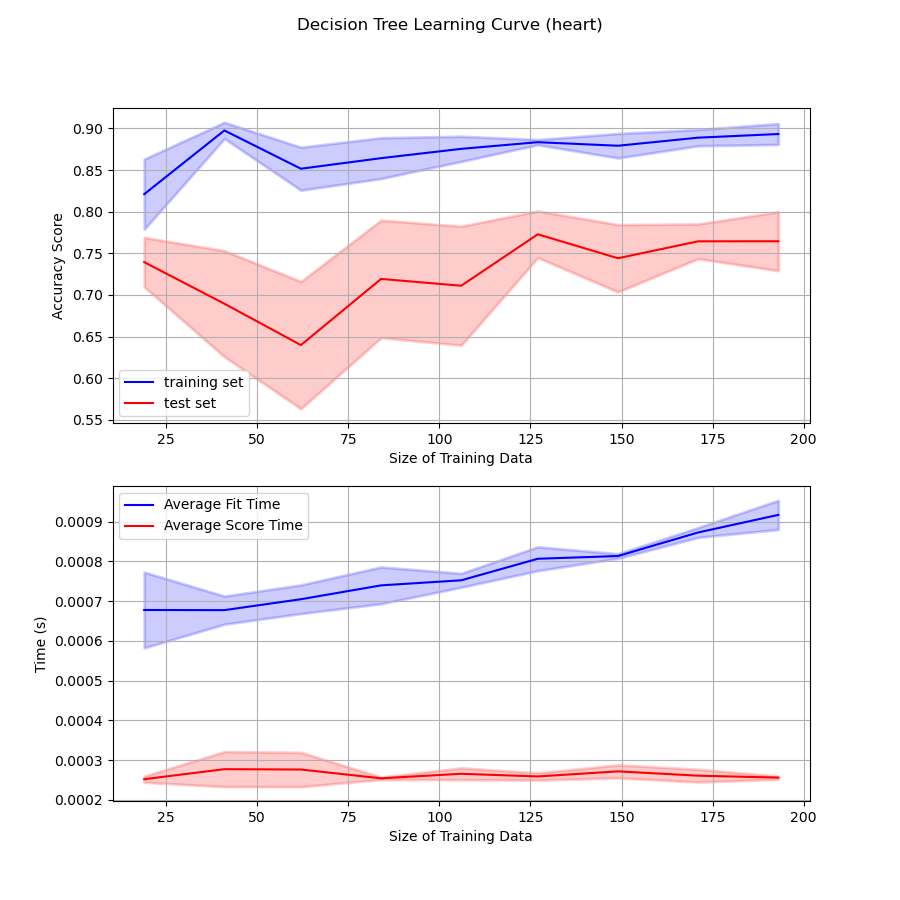
\includegraphics[width=0.40\textwidth]{../outputs/DT_LearningCurve_heart.png}}}
	\subfigure[]{\frame{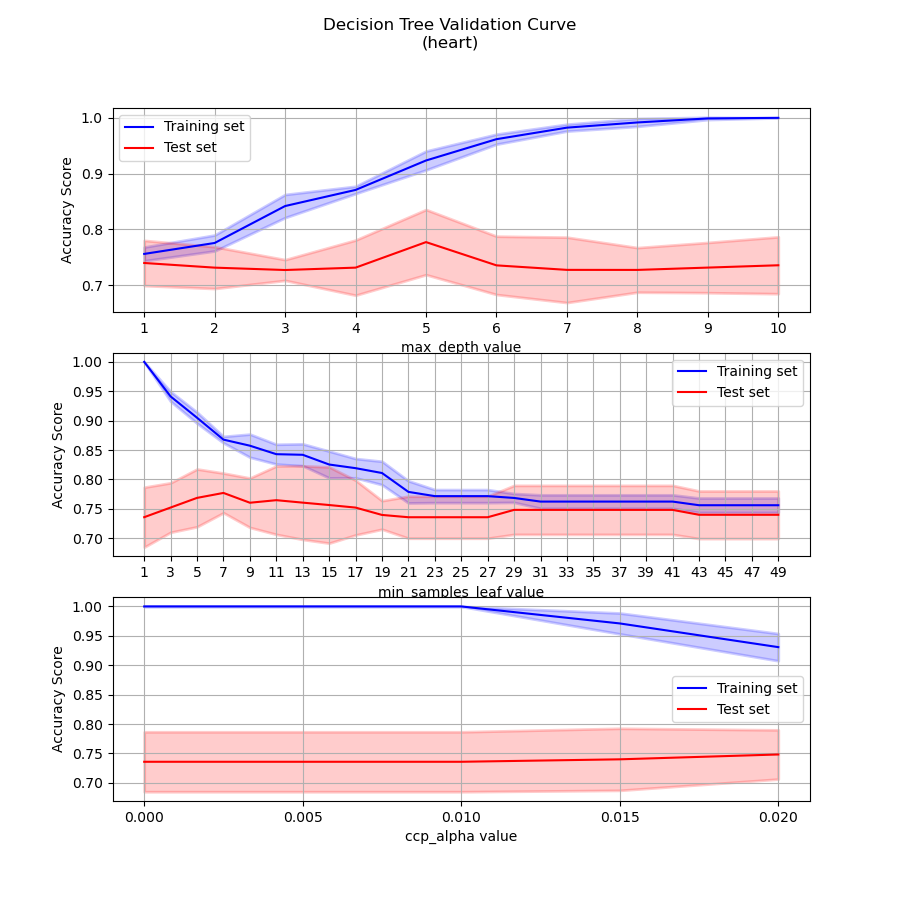
\includegraphics[width=0.40\textwidth]{../outputs/DT_ValidationCurve_heart.png}}}
	\caption{Decision Tree Model trained on the Heart dataset. (a) Learning Curve and (b) Validation Curve}
	\label{fig:fig4}
\end{figure}

In the learning curve, you can see clearly that for both datasets, the cross-validation accuracy increases as the training set increases. This means that both datasets are a little bit on the small side and could be improved by adding more data. Water potiblity is about 10 times the size of the heart dataset, but considering the fact that it has continuous features, it makes sense that it would be a little harder to classify.

The three parameters that I chose to optimize for DTs are max depth, min leaf size, and ccp alpha. Max depth limits how many splits down the tree can go before it must have a leaf node. Leaf size is similar in that it requires the tree to produce a leaf, but rather than constraining the depth of the tree, it constrains the size of the leaf. Each leaf must be no smaller than this parameter. Lastly is ccp alpha, which, from the sklearn docs, is a "Complexity parameter used for Minimal Cost-Complexity Pruning." It is a factor of post training pruning to reduce size and generalize better.

The reason I chose these three parameters are because they are the primary factors in determining how tightly the model fits to the data. They are all factors of pruning, although they each handle it in different ways. From the validation curves, you can see that max depth doesn't exactly have a direct correlation to accuracy, with both models peaking at different points. Similarly with leaf size, as the size increases, the training accuracy goes down, but the test accuracy slightly goes up, because it creates a more generalized model, rather than an overfitted model. The ccp alpha value causes a steep reduction in training accuracy, but a slight increase in test accuracy, although not much.

It should not be a surprise then that both both datasets, the optimal parameters were somewhere in the middle for max depth, relatively low for min leaf size, and low for ccp alpha, since the alpha value had a more significant effect on overall accuracy.

\subsection{AdaBoost}
AdaBoost is an ensamble learner, meaning it is a combination of multiple weak learners. In this implementation, it is a combination of a series of decision trees with high pruning. I used a somewhat arbitrary default decision tree so that I could focus my analysis on the Boosting model itself rather than the DT. For this reason, I kept the DT fixed with a max depth of 3, and varied the number of estimators and the learning rate. Boosting is a very useful model because it can take the strengths of a model such as decision trees, but by combining several of them together, it is able generalize better and reduces the amount of overfitting. This comes at a cost of speed. Since there are multiple decision trees being trained and used for prediction, it makes them much slower than decision trees, although still faster than some others.

% accuracy table
\begin{center}
	\begin{tabular}{|c||c|c|}
	 \hline
	  & Cross Validation Score & Test Accuracy \\
	 \hline\hline
	 Water Dataset & 64.1\%  & 63.8\% \\
	 \hline
	 Heart Dataset & 80.2\%  & 80.3\% \\
	 \hline
	\end{tabular}
	\label{table:table2}
\end{center}
% Boost plots - Water
\begin{figure}
	\centering
	\subfigure[]{\frame{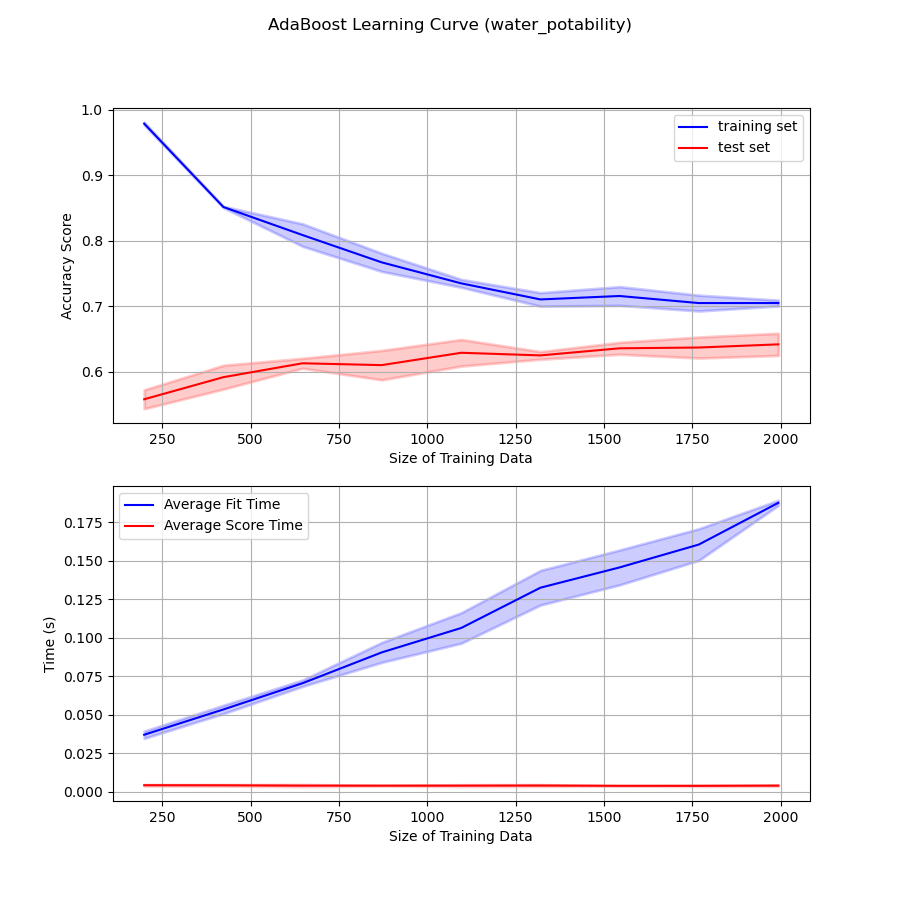
\includegraphics[width=0.40\textwidth]{../outputs/Boost_LearningCurve_water_potability.png}}}
	\subfigure[]{\frame{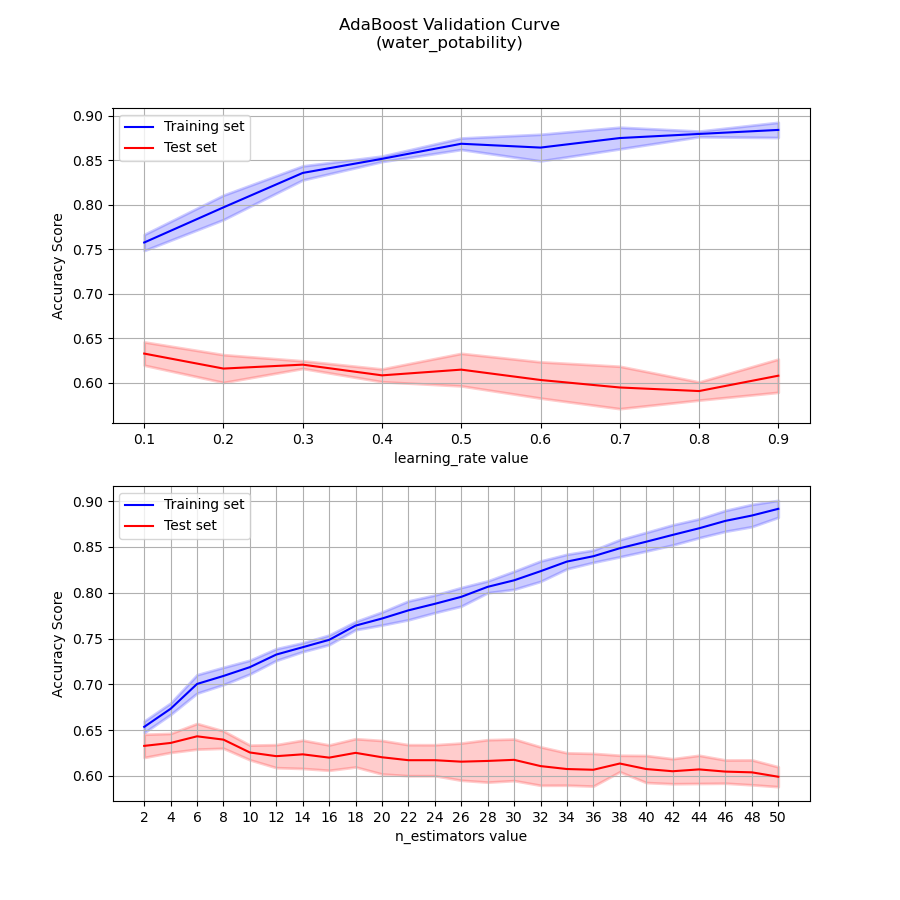
\includegraphics[width=0.40\textwidth]{../outputs/Boost_ValidationCurve_water_potability.png}}}
	\caption{AdaBoost Model trained on water potability dataset. (a) Learning Curve and (b) Validation Curve}
	\label{fig:fig5}
\end{figure}
% Boost plots - Heart
\begin{figure}
	\centering
	\subfigure[]{\frame{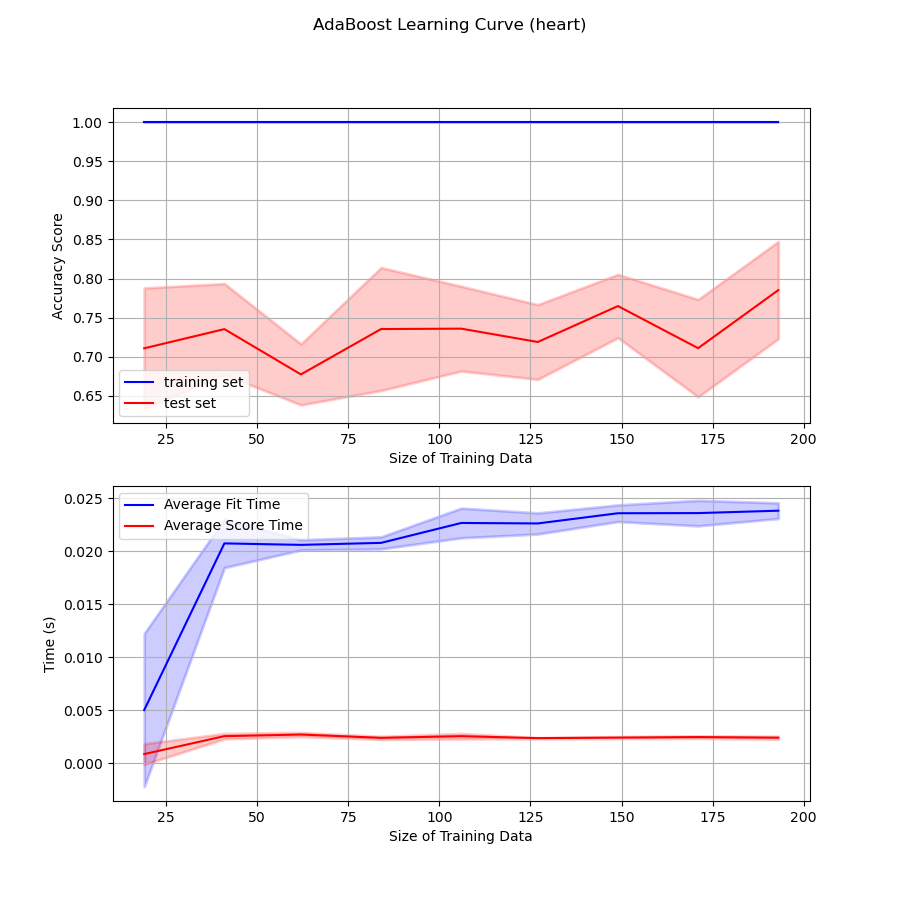
\includegraphics[width=0.40\textwidth]{../outputs/Boost_LearningCurve_heart.png}}}
	\subfigure[]{\frame{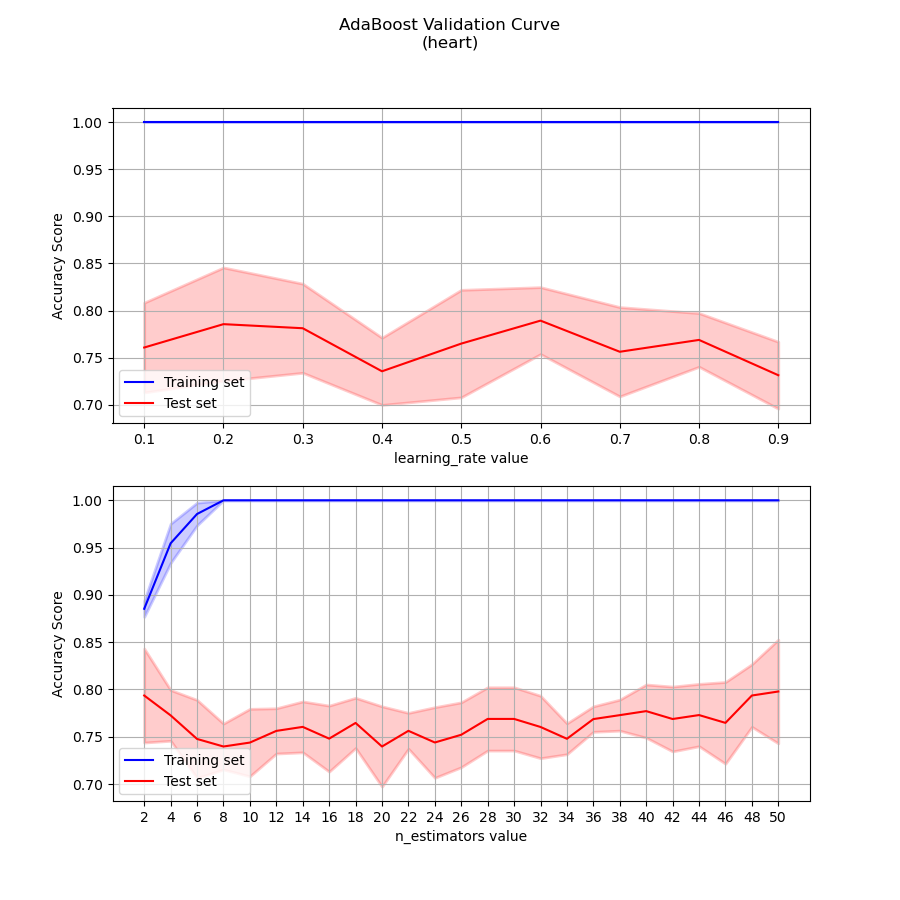
\includegraphics[width=0.40\textwidth]{../outputs/Boost_ValidationCurve_heart.png}}}
	\caption{AdaBoost Model trained on heart dataset. (a) Learning Curve and (b) Validation Curve}
	\label{fig:fig6}
\end{figure}

AdaBoost performed just slightly better than decision trees on both datasets, and had the best generalized representation of all 5 models tested. Both the training and test accuracy was less than 0.5\% different between the two. Just as with decision trees, the learning curve shows that the higher the amount of training data, the better the performance. This means that either the datasets are too small, or that both DT and Boosting require a lot of data to perform well.

The two main parameters when designing a Boosting model are the number of estimators, and the learning rate. The number of estimators is obviously the number of instances of the DT model, and the learning rate is the weight applied to each iteration. It primarily affects how quickly the model learns, although can have an affect on accuracy as well. ALthough not plotted here, higher learning rate makes the model converge more quickly, but as you can see in the validation curve, it also tends to be less accurate. One would expect that higher values for estimators, and lower values of learning rate would be optimal. In both datasets, the models converged at estimators in the low 20s and learning rates at 0.5 or less.

\subsection{Neural Networks}
% TODO


% accuracy table
\begin{center}
	\begin{tabular}{|c||c|c|}
	 \hline
	  & Cross Validation Score & Test Accuracy \\
	 \hline\hline
	 Water Dataset & 67.9\%  & 39.6\% \\
	 \hline
	 Heart Dataset & 83.9\%  & 73.8\% \\
	 \hline
	\end{tabular}
	\label{table:table3}
\end{center}
% Neural Net Plots - Water
\begin{figure}
	\centering
	\subfigure[]{\frame{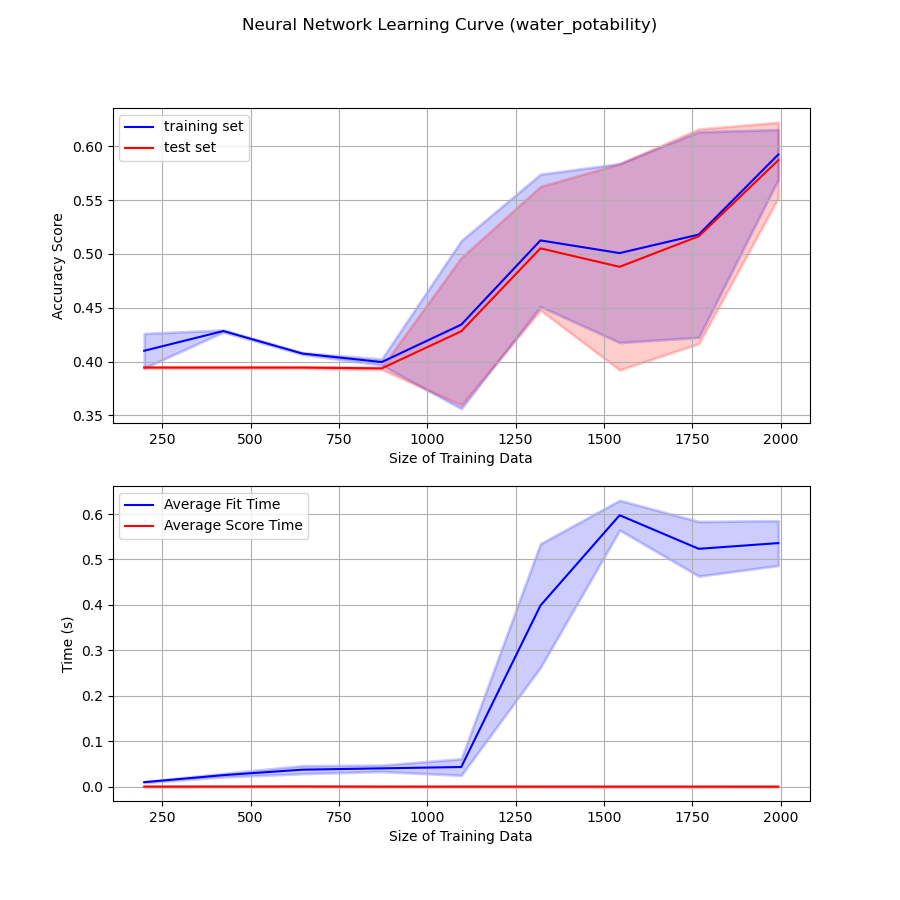
\includegraphics[width=0.40\textwidth]{../outputs/NN_LearningCurve_water_potability.png}}}
	\subfigure[]{\frame{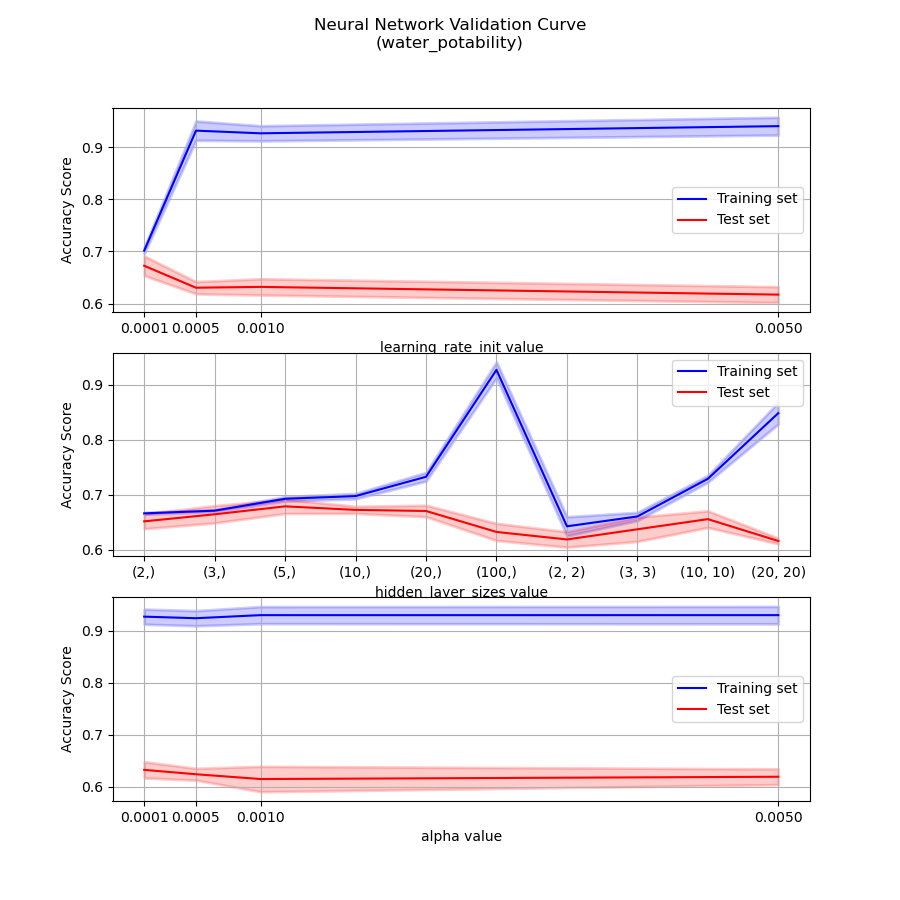
\includegraphics[width=0.40\textwidth]{../outputs/NN_ValidationCurve_water_potability.png}}}
	\caption{Neural Network Model trained on water potability dataset (a) Learning Curve and (b) Validation Curve}
	\label{fig:fig6}
\end{figure}
% Neural Net Plots - heart
\begin{figure}
	\centering
	\subfigure[]{\frame{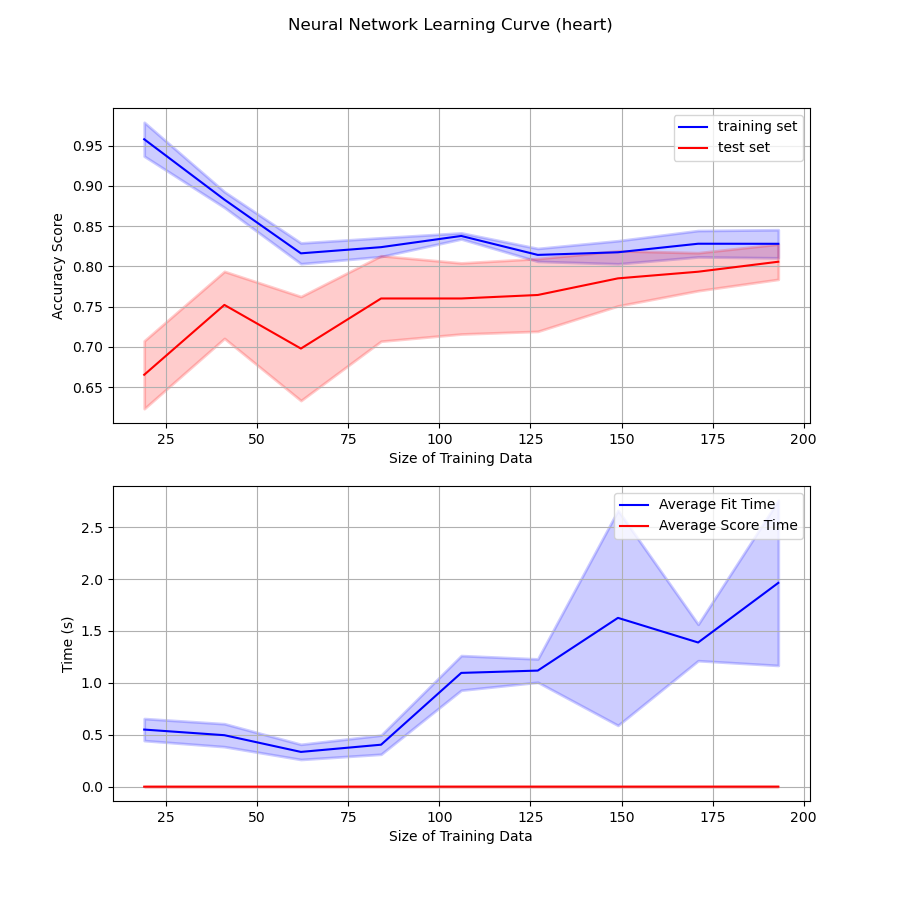
\includegraphics[width=0.40\textwidth]{../outputs/NN_LearningCurve_heart.png}}}
	\subfigure[]{\frame{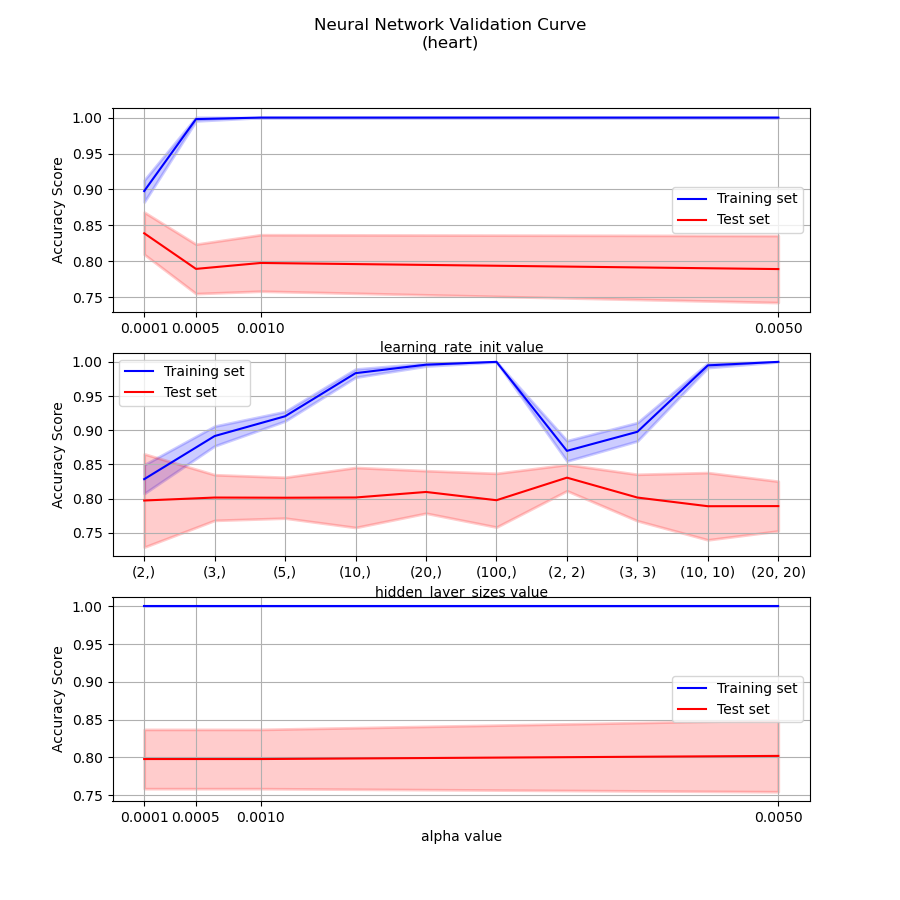
\includegraphics[width=0.40\textwidth]{../outputs/NN_ValidationCurve_heart.png}}}
	\caption{Neural Network Model trained on heart dataset (a) Learning Curve and (b) Validation Curve}
	\label{fig:fig8}
\end{figure}
% Neural Net Plots - Loss
\begin{figure}
	\centering
	\subfigure[]{\frame{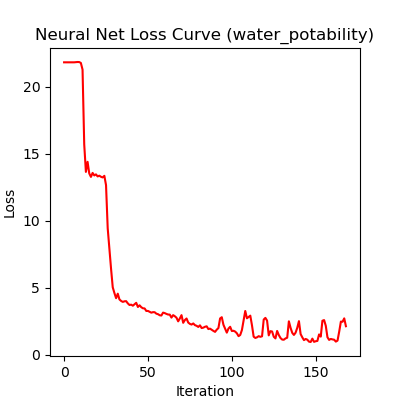
\includegraphics[width=0.40\textwidth]{../outputs/NN_LossGraph_water_potability.png}}}
	\subfigure[]{\frame{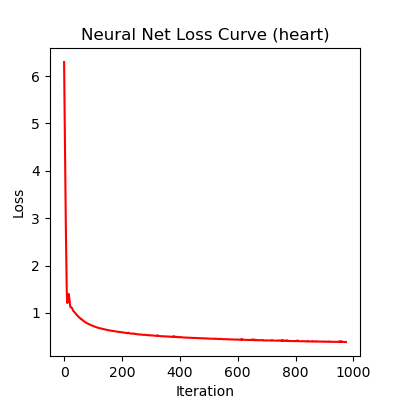
\includegraphics[width=0.40\textwidth]{../outputs/NN_LossGraph_heart.png}}}
	\caption{Neural Network Loss graph for: (a) water potability dataset and (b) heart dataset}
	\label{fig:fig9}
\end{figure}


\subsection{Support Vector Machines}
% TODO


% accuracy table
\begin{center}
	\begin{tabular}{|c||c|c|}
	 \hline
	  & Cross Validation Score & Test Accuracy \\
	 \hline\hline
	 Water Dataset & 67.3\%  & 61.8\% \\
	 \hline
	 Heart Dataset & 84.7\%  & 70.5\% \\
	 \hline
	\end{tabular}
	\label{table:table4}
\end{center}
% SVM Plots - water
\begin{figure}
	\centering
	\subfigure[]{\frame{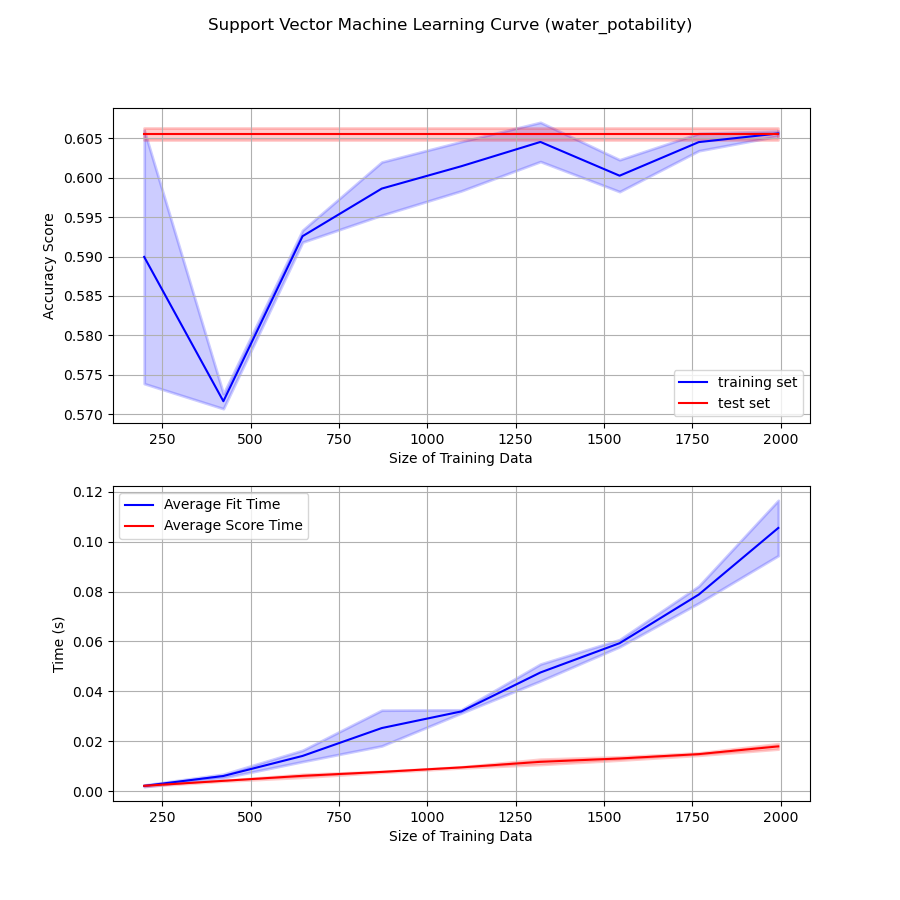
\includegraphics[width=0.40\textwidth]{../outputs/SVM_LearningCurve_water_potability.png}}}
	\subfigure[]{\frame{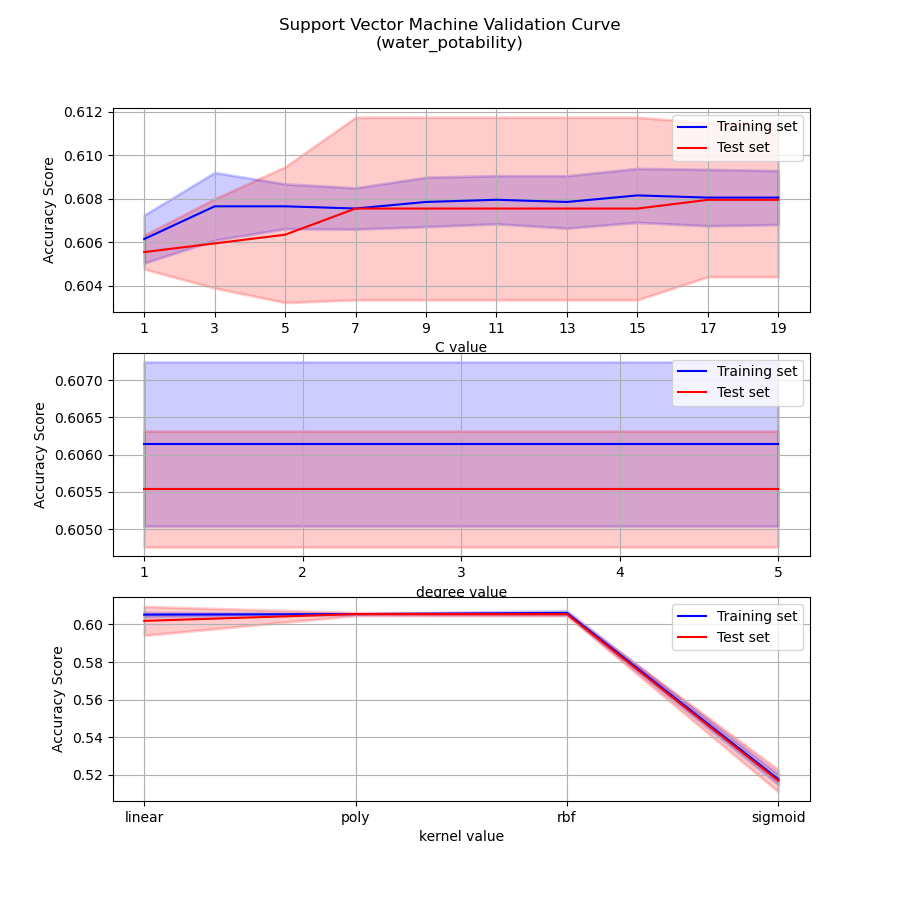
\includegraphics[width=0.40\textwidth]{../outputs/SVM_ValidationCurve_water_potability.png}}}
	\caption{SVM Model trained on water potability dataset. (a) Learning Curve and (b) Validation Curve}
	\label{fig:fig10}
\end{figure}
% SVM Plots - heart
\begin{figure}
	\centering
	\subfigure[]{\frame{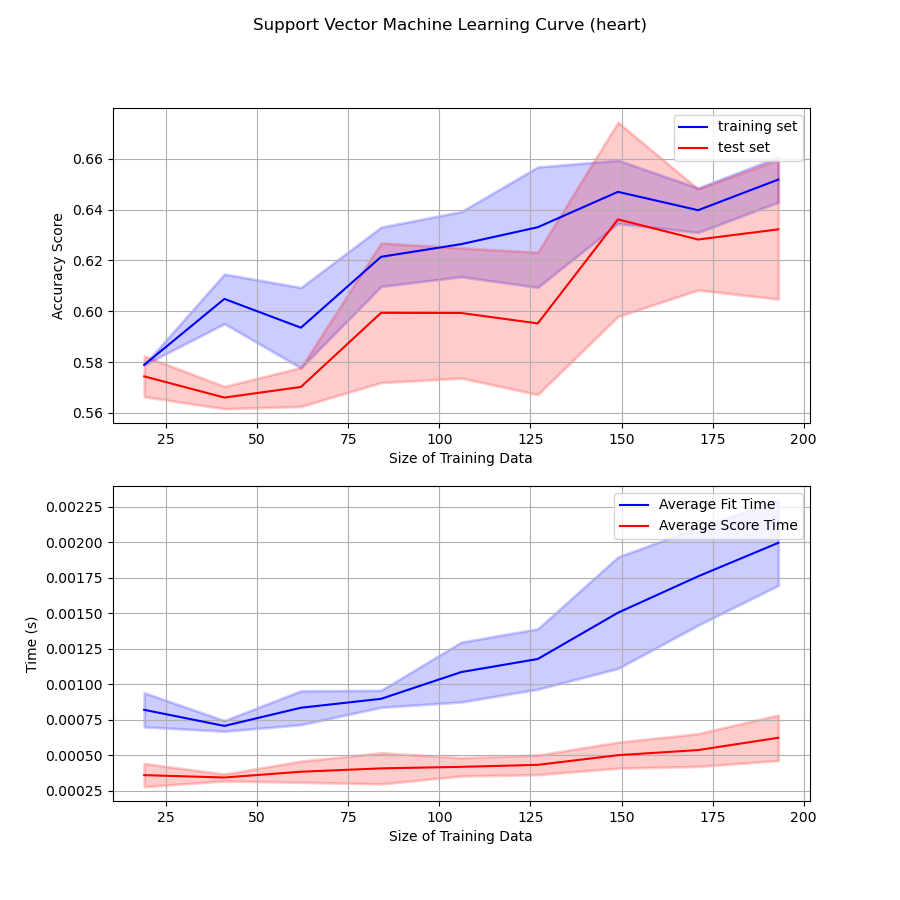
\includegraphics[width=0.40\textwidth]{../outputs/SVM_LearningCurve_heart.png}}}
	\subfigure[]{\frame{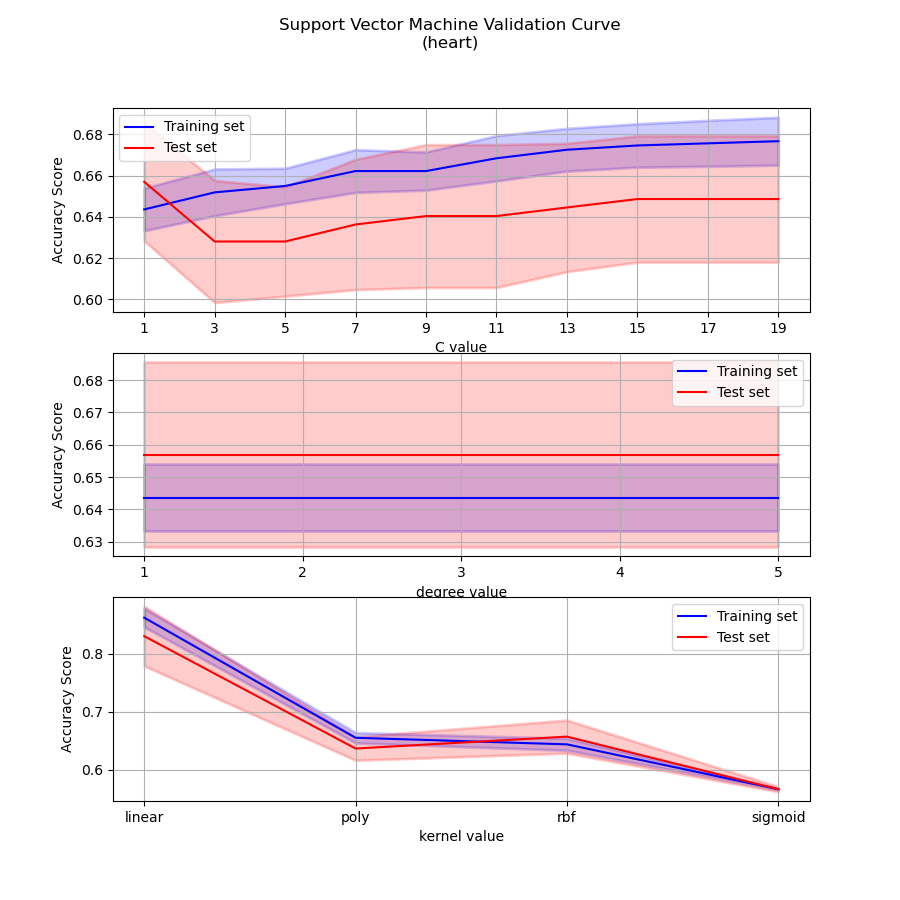
\includegraphics[width=0.40\textwidth]{../outputs/SVM_ValidationCurve_heart.png}}}
	\caption{SVM Model trained on heart dataset. (a) Learning Curve and (b) Validation Curve}
	\label{fig:fig11}
\end{figure}

\subsection{K-Nearest Neighbor}
% TODO


% accuracy table
\begin{center}
	\begin{tabular}{|c||c|c|}
	 \hline
	  & Cross Validation Score & Test Accuracy \\
	 \hline\hline
	 Water Dataset & 64.8\%  & 57.4\% \\
	 \hline
	 Heart Dataset & 84.7\%  & 73.8\% \\
	 \hline
	\end{tabular}
	\label{table:table5}
\end{center}
% KNN Plots - water
\begin{figure}
	\centering
	\subfigure[]{\frame{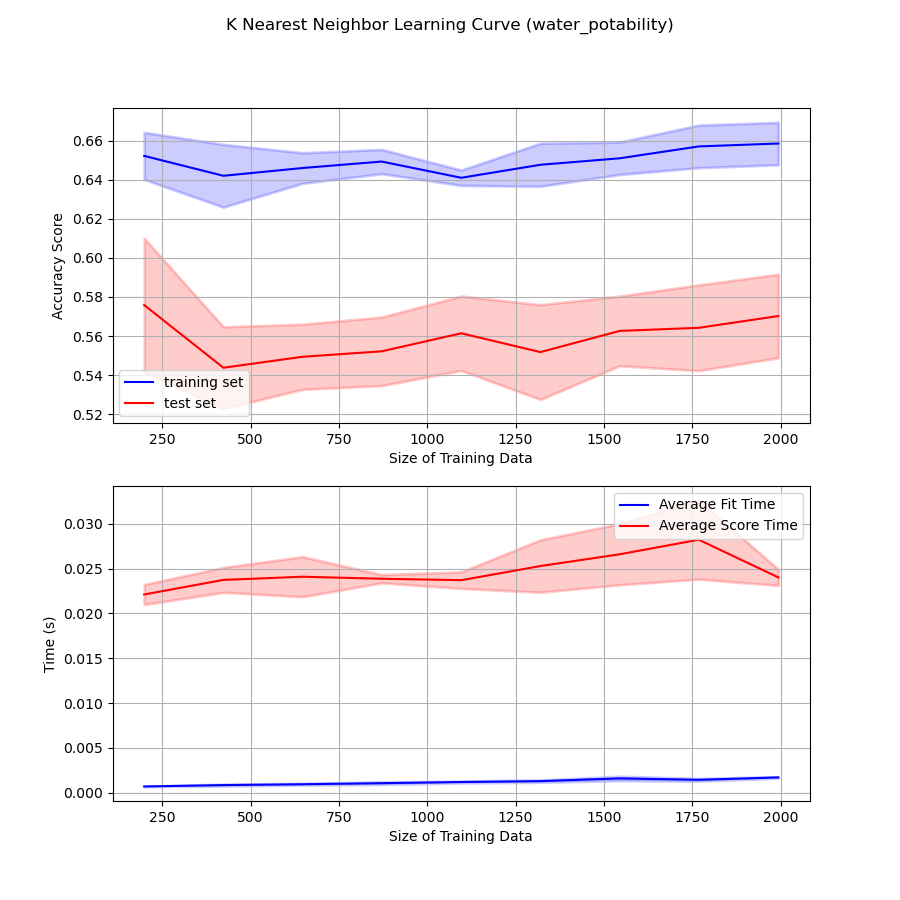
\includegraphics[width=0.40\textwidth]{../outputs/KNN_LearningCurve_water_potability.png}}}
	\subfigure[]{\frame{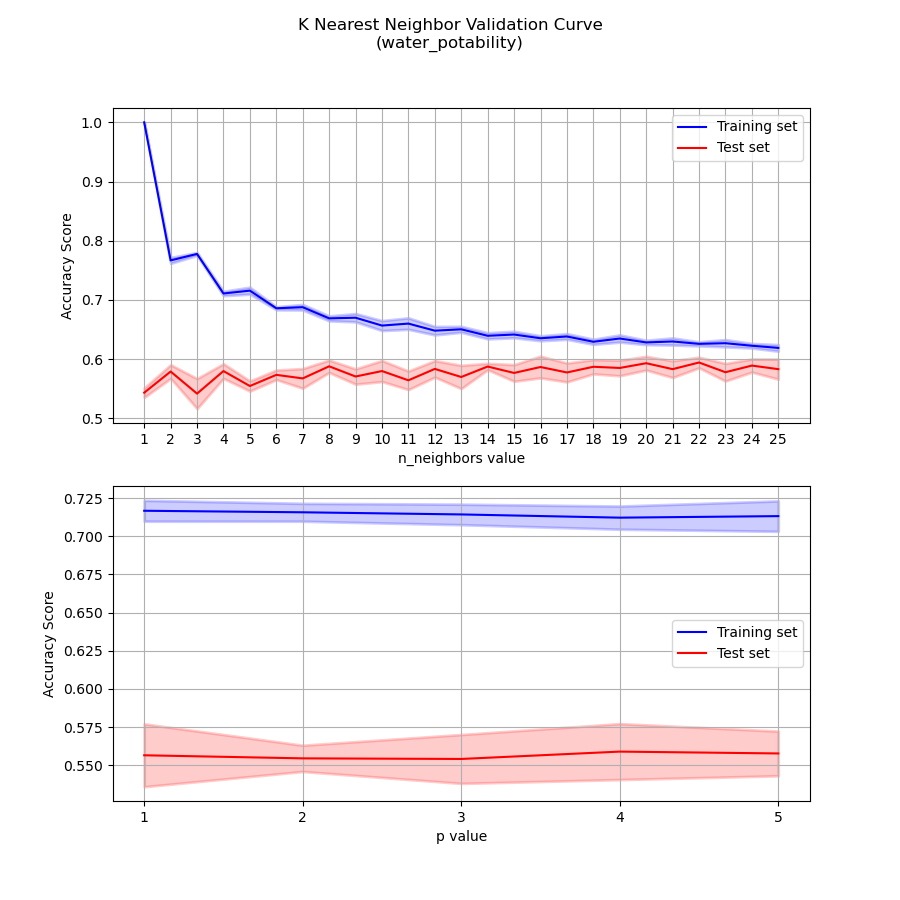
\includegraphics[width=0.40\textwidth]{../outputs/KNN_ValidationCurve_water_potability.png}}}
	\caption{KNN Model trained on water potability dataset. (a) Learning Curve and (b) Validation Curve}
	\label{fig:fig12}
\end{figure}
% KNN Plots - water
\begin{figure}
	\centering
	\subfigure[]{\frame{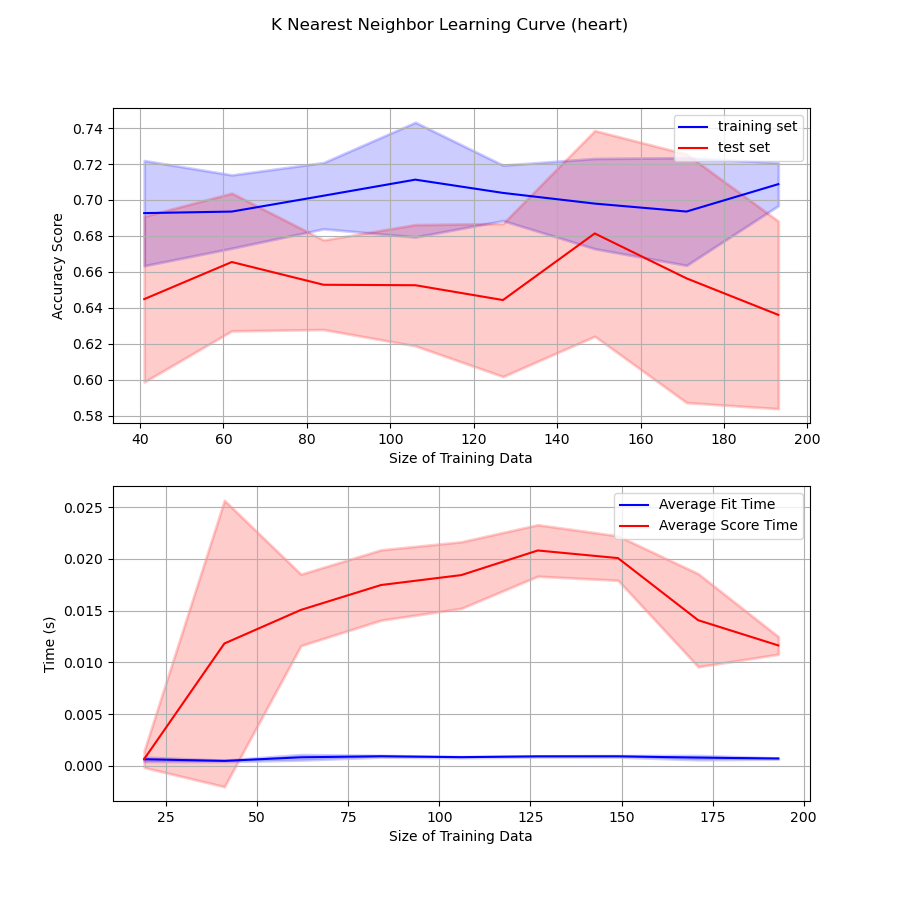
\includegraphics[width=0.40\textwidth]{../outputs/KNN_LearningCurve_heart.png}}}
	\subfigure[]{\frame{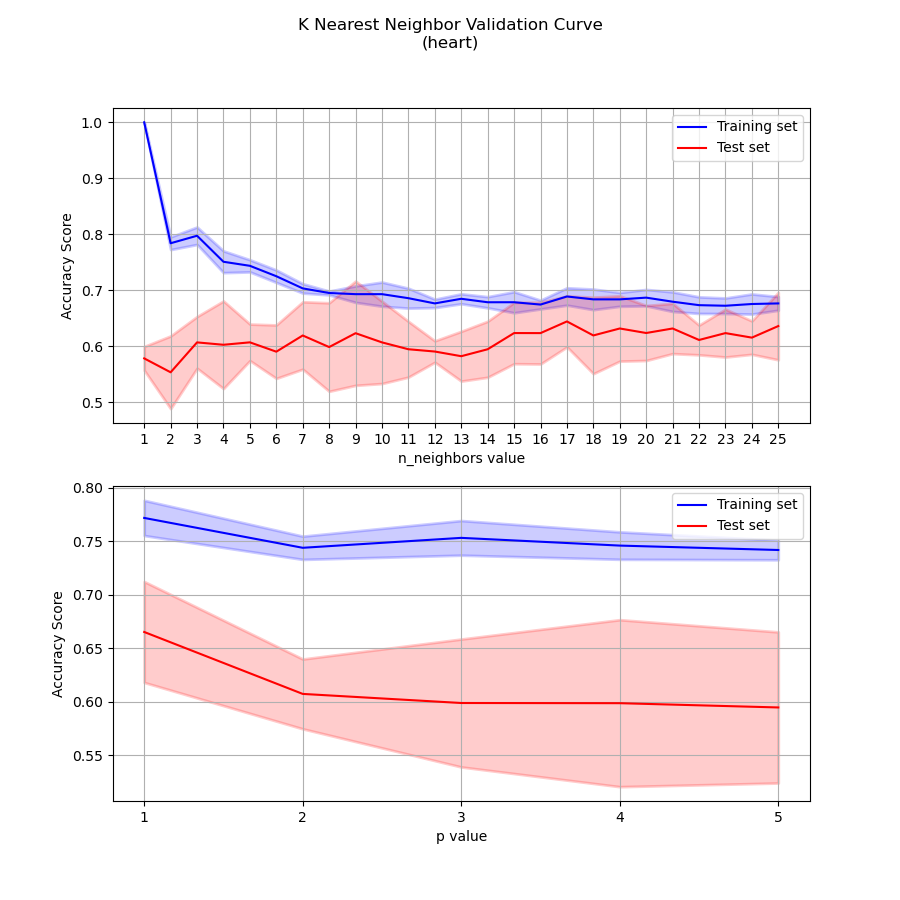
\includegraphics[width=0.40\textwidth]{../outputs/KNN_ValidationCurve_heart.png}}}
	\caption{KNN Model trained on heart dataset. (a) Learning Curve and (b) Validation Curve}
	\label{fig:fig13}
\end{figure}



% \begin{table}[h] % [h] forces the table to be output where it is defined in the code (it suppresses floating)
% 	\caption{Mathematical constants. Notice how the approximations align at the decimal.}
% 	\small % Reduce font size
% 	\centering % Centre the table
% 	\begin{tabular}{L{0.17\linewidth} C{0.12\linewidth} L{0.17\linewidth} L{0.4\linewidth}}
% 		\textbf{Name} & \textbf{Symbol} & \textbf{Approximation} & \textbf{Description} \\
% 		\toprule[0.5pt]
% 		Golden ratio & $\phi$ & 1.618 & Number such that the ratio of " to the number is equal to the ratio of its reciprocal to 1\\
% 		\midrule
% 		Euler's number & $e$ & 2.71828 & Exponential growth constant\\
% 		\midrule
% 		Archimedes' constant & $\pi$ & 3.14 & The ratio between circumference and diameter of a circle\\
% 		\midrule
% 		One hundred & A+ & 100.00 & The grade we hope you’ll all earn in this class\\
% 	\end{tabular}
% \end{table}


\newpage

\section{References}
\printbibliography

\end{document}